\documentclass[a5paper,12pt]{article}
\usepackage{amssymb, amsfonts, fancyhdr, tikz, helvet, svg, titlesec, pdfpages, pdflscape, rotating}
\usepackage[left=2.3cm,right=2.3cm,top=3cm,headsep=2cm]{geometry}

\begin{document}
\renewcommand{\familydefault}{helvet}
\renewcommand{\familydefault}{\ttdefault}

\titleformat*{\section}{\Large \ttfamily}

\pagestyle{fancy}
\fancyhf{}

\fancyhead[C]{
\includegraphics[width=1cm]{Logatronik.pdf}}
\fancyfoot[C]{\thepage}
%\fancyfoot[L]{\Large MCHID Type A [En/De]}

\renewcommand{\headrulewidth}{0pt}

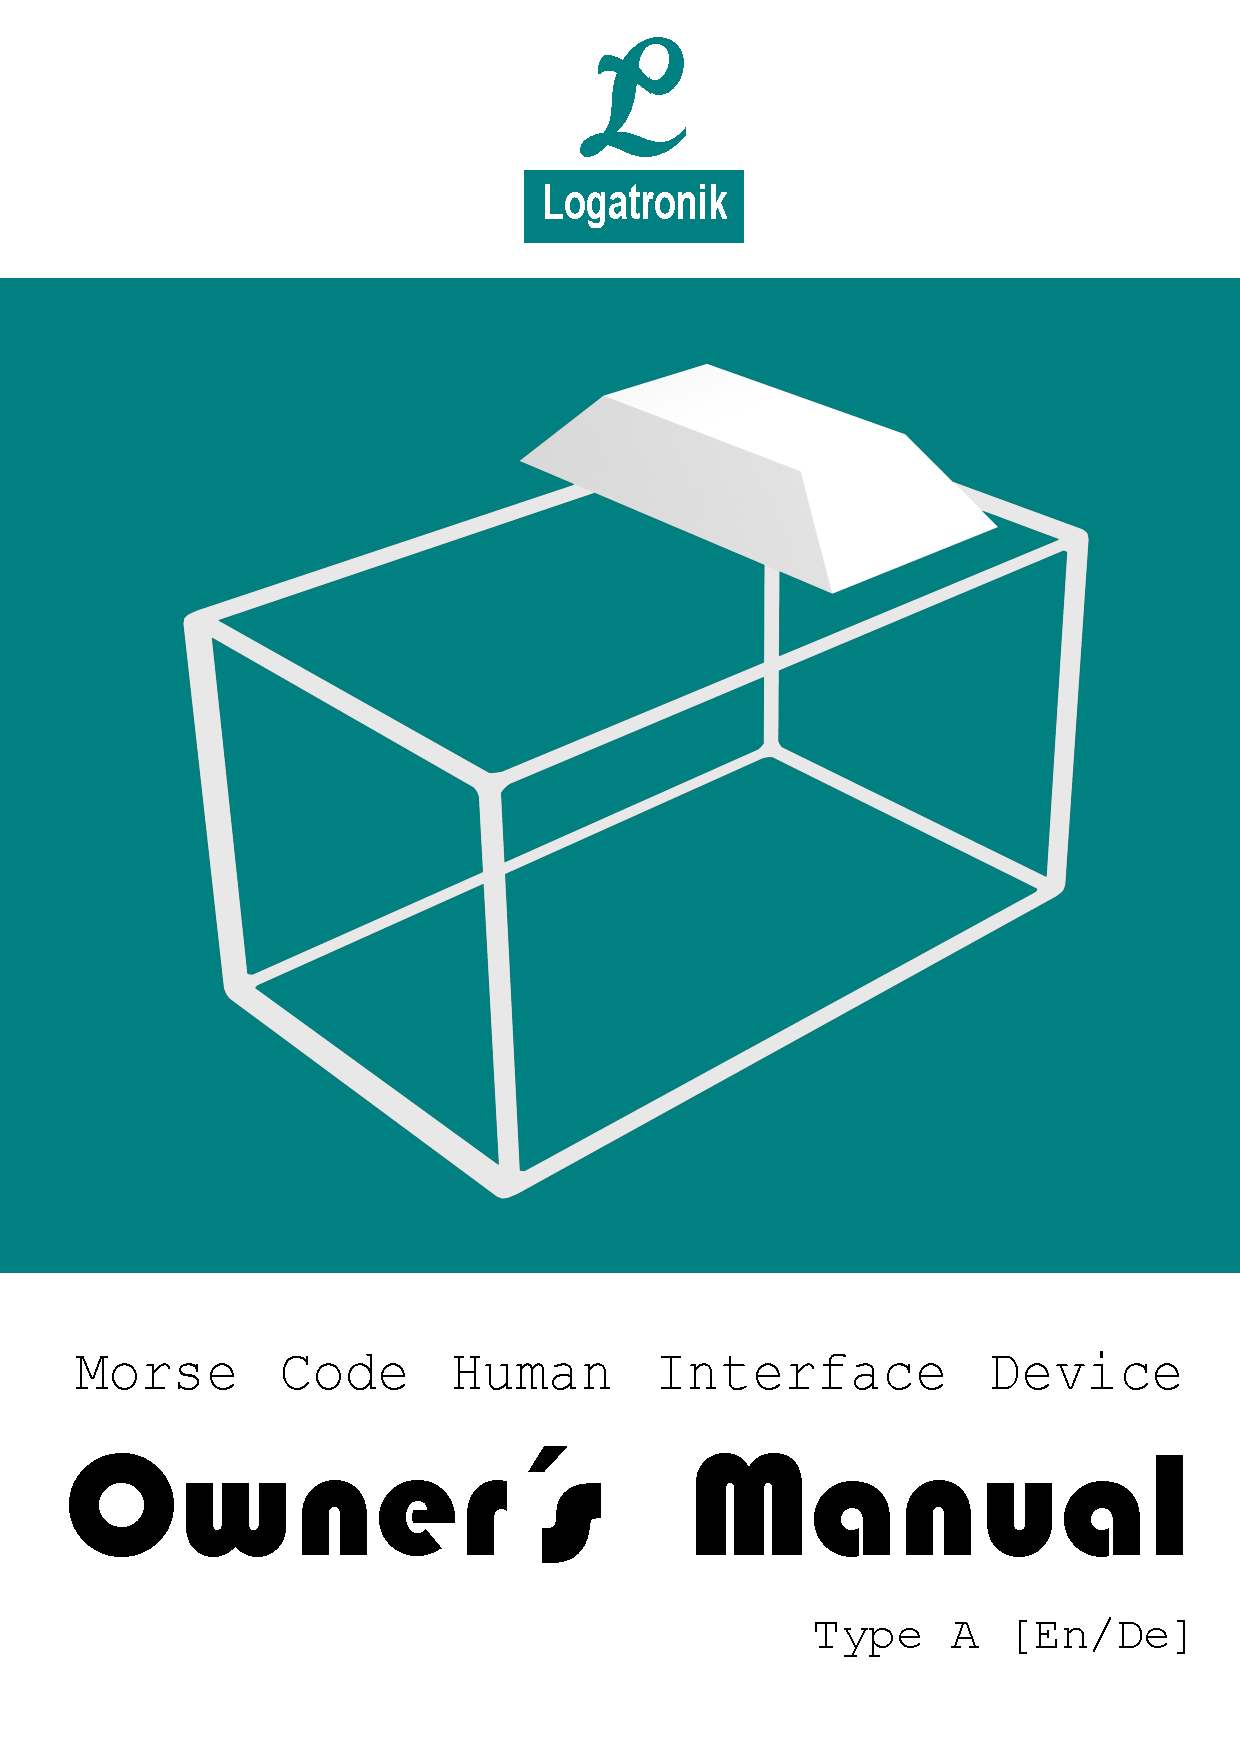
\includepdf[pages=-]{FrontPage.pdf}
\newpage
\setcounter{page}{1}
    
    \tableofcontents{}
    \section{Welcome!}
    The Morse Code Human Interface Device let's you use the full power of \emph{morse code} on your computer;
    Be no longer slave to the over engineered keyboard and enjoy true minmalism with MCHID!\\
    Thank you for choosing Logatronik to dive into this brave new world of oneness with the digital.\\

    \section{Installation}\label{installation}
    To install the device simply connect it with a pc. The drivers should automatically be installed.
    Due to technical limitations \"A, \"O, \"U are only supported when the computer is set to the US keyboard or similar and might lead to unexpected results otherwise. 
    \section{The Morse Code used}
    The code used is mostly the same as the ITU\footnote{International Telecommunication Union} standard, with the addition of German letters, though their support is limited (see section~\ref{installation}). The exact translations can be extracted from figure~\ref{fig:morseTree} on page~\ref{morseTree}.

    \begin{description}

        \item[Dot-time:] The maximal duration for a dot is about 170ms
        \item[Dash-time:] The maximal duration for a dash is three times that of a dot
        \item[Deletion:] If the length of an input sequence for a single character exceeds 6, the MCHID will delete the previous letter for any further press of the button, until there is no further input for the duration of a dash.
        \item[Space:] There are two options for spaces (see section~\ref{modifications} on how to select them).
            \begin{description}
            \item[Long Press:] By pressing the button longer than a dash-time a space is written.
            \item[Timed:] After the duration of 7 dots with no input a space is written.
            \end{description}
    \end{description}
            
    \begin{center}
    \label{morseTree}
    \begin{sidewaysfigure}[h]
    
\begin{tikzpicture}[level 1/.style={sibling distance=8cm}, level 2/.style={sibling distance=4cm}, level 3/.style={sibling distance=2cm}, level 4/.style={sibling distance=1cm}, level 5/.style={sibling distance=5mm}]
\node (start) {start}
child {node (E) {E} edge from parent[dashed]
    child {node (I) {I} edge from parent[dashed]
            child {node (S) {S} edge from parent[dashed]
                child {node (H) {H} edge from parent[dashed]
                    child {node (5) {5} edge from parent[dashed]}
                    child {node (4) {4} edge from parent[solid]}
                }
               child {node (V) {V} edge from parent[solid]
                    child {node (empty) {} edge from parent[dashed]}
                    child {node (3) {3} edge from parent[solid]}
                    }
            }
            child {node (U) {U} edge from parent[solid]
                child {node (F) {F} edge from parent[dashed]
                    child {node (dot) {.} edge from parent[dashed]}
                    child {node (comma) {,} edge from parent[solid]}
                }
                child {node ("U) {"U} edge from parent[solid]
                    child {node (empty) {} edge from parent[dashed]}
                    child {node (2) {2} edge from parent[solid]}
               }
            }
       }
    child {node (A) {A} edge from parent[solid]
            child {node (R) {R} edge from parent[dashed]
                child {node (L) {L} edge from parent[dashed]
                    child {node (empty) {} edge from parent[dashed]}
                    child {node (empty) {} edge from parent[solid]}
               }
                child {node ("A) {"A} edge from parent[solid]
                    child {node (sign+) {+} edge from parent[dashed]}
                    child {node (sign-) {-} edge from parent[solid]}
                }
            }
            child {node (W) {W} edge from parent[solid]
               child {node (P) {P} edge from parent[dashed]
                    child {node (empty) {} edge from parent[dashed]}
                    child {node (empty) {} edge from parent[solid]}
               }
               child {node (J) {J} edge from parent[solid]
                    child {node (empty) {} edge from parent[dashed]}
                    child {node (1) {1} edge from parent[solid]}
               }
            }
        }
    }
child {node (T) {T} edge from parent[solid]
    child {node (N) {N} edge from parent[dashed]
        child {node (D) {D} edge from parent[dashed]
            child {node (B) {B} edge from parent[dashed]
                child {node (6) {6} edge from parent[dashed]}
                child {node (=) {=} edge from parent[solid]}
            }
            child {node (X) {X} edge from parent[solid]
                child {node (/) {/} edge from parent[dashed]}
                child {node (*) {*} edge from parent[solid]}
            }
          }
          child {node (K) {K} edge from parent[solid]
            child {node (C) {C} edge from parent[dashed]
                child {node (empty) {} edge from parent[dashed]}
                child {node (enter) {ENT} edge from parent[solid]}
            }
            child {node (Y) {Y} edge from parent[solid]
                child {node (empty) {} edge from parent[dashed]}
                child {node (empty) {} edge from parent[solid]}
            }
          }
     }
    child {node (M) {M} edge from parent[solid]
        child {node (G) {G} edge from parent[dashed]
            child {node (Z) {Z} edge from parent[dashed]
                child {node (7) {7} edge from parent[dashed]}
                child {node (empty) {} edge from parent[solid]}
            }
            child {node (Q) {Q} edge from parent[solid]
                child {node (empty) {} edge from parent[dashed]}
                child {node (empty) {} edge from parent[solid]}
            }
            }
        child {node (O) {O} edge from parent[solid]
            child {node ("O) {"O} edge from parent[dashed]
                child {node (8) {8} edge from parent[dashed]}
                child {node (empty) {} edge from parent[solid]}
            }
            child {node (" ") {" "} edge from parent[solid]
                child {node (9) {9} edge from parent[dashed]}
                child {node (0) {0} edge from parent[solid]}
            }
            }
        }
    }
;

\path (start) -- (E)[dotted];
\path (start) -- (T)[dotted];

\end{tikzpicture}

        \caption{The Tree of the implemented code}
        \label{fig:morseTree}
    \end{sidewaysfigure}
    \end{center}
    \section{Modifications}\label{modifications}
    There is already support in the MCHID for some customization, though the intrigued might want to go further; your imagination is the only limit!

\end{document}
